
\chapter{Heurística GRASP}\label{grasp}
Neste capítulo é feita uma revisão bibliografica da heurística GRASP, bem como sua fase de construção e de busca local.

\section{Introdução}
GRASP - {\it Greedy Randomized Adaptive Search Procedure}, ou procedimento de busca adaptativa gulosa e aleatória, é uma técnica iterativa proposta por \citeonline{FEO_REZENDE} que consiste numa fase de construção de uma solução viável, na qual uma solução é gerada, elemento a elemento, e de uma fase de busca local, na qual se procura melhorar de forma iterativa a qualidade da solução encontrada anteriormente, a fase de busca local trabalha de forma iterativa através de sucessivas substituições da solução atual por uma melhor de sua vizinhança, quando não há mais soluções melhores essa fase é terminada.

Na figura \ref{proc_grasp}, encontra-se um pseudocógico genérico da heurística GRASP, os parâmetros que precisam ser definidos na heurísitca são o parâmetro de aleatoriedade $\alpha$ e o critério de parada (GRASPmax) que geralmente é o numero de iterações da heurística. De acordo com a figura \ref{proc_grasp}, a heurística GRASP constrói repetidamente uma solução (passo 4) e esta é melhorada por uma busca local (passo 5) e a melhor solução encontrada até o momento é armazenada (passo 7 e 8).

A melhor solução encontrada ao longo de todas as interações GRASP realizadas é retornada como resultado do algoritmo de otimização GRASP \cite{SOUZA}

%\begin{figure}[H]
%\centering
%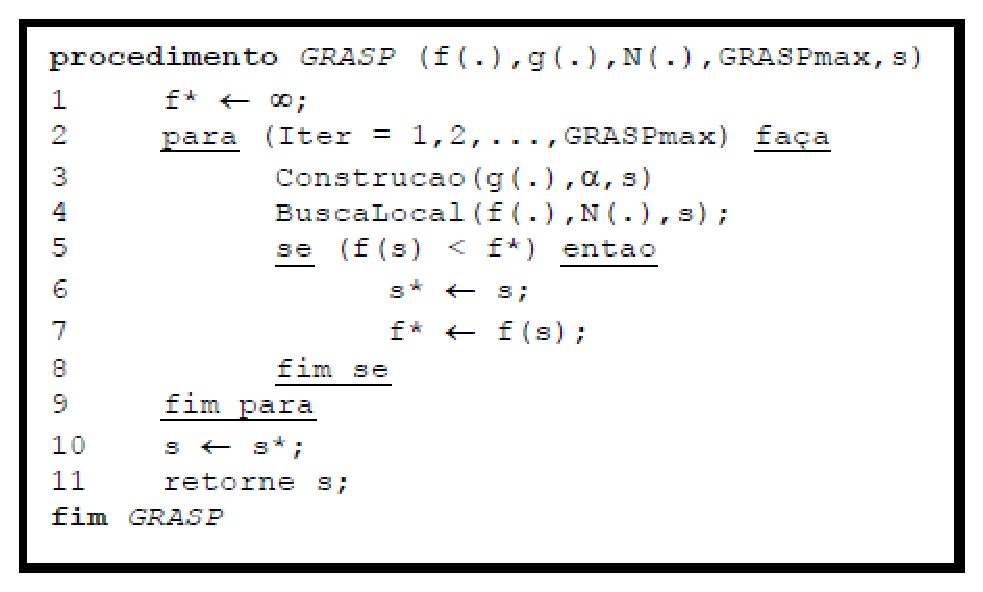
\includegraphics[scale = 0.8]{graficos/grasp.eps}  
%\caption{Pseudo-código da heurística GRASP}
%\label{proc_grasp}
%\end{figure}

\begin{figure}[H]
    \begin{center}
       \begin{tabular}{c} \hline
        \begin{lstlisting}[mathescape] 
	${\it procedimento}$ GRASP (f(.), g(.), N(.), GRASPmax, s)
	$f^{*} \leftarrow \infty$;
	${\it para}$ (iter = 1,2, ..., GRASPmax) ${\it faca}$
		$\quad$Construcao(g(.), $\alpha$, s);
		$\quad$BuscaLocal(f(.), N(.), s);
		${\it se}$ (f(s) < $f^{*}$ ${\it entao}$
			$\quad s^{*} \leftarrow s$;
			$\quad f^{*} \leftarrow f(s)$;
		${\it fim se}$
	${\it fim para}$
	s $\leftarrow s^{*}$;
	${\it retorne}$ s;
	${\it fim}$ GRASP
	
	\end{lstlisting}

\\
\hline
 \end{tabular}
 \end{center}
\caption{Pseudo-código da heurística GRASP}
\label{proc_grasp}
 \end{figure}

Como o GRASP normalmente trata de problemas da ordem de complexidade NP-Dificil, poderia ficar indefinidamente em busca de uma solução ótima, para evitar esse caso, é preciso adotar um critério de parada na fase de busca local, por exemplo, o número máximo de iterações.

\section{Fase Construtiva}\label{teste}
Na fase de construção, uma solução é iterativamente construída, elemento por elemento. A cada iteração dessa fase, os próximos elementos candidatos a serem incluídos na solução são colocados em uma lista C de candidatos, seguindo um critério de ordenação pré-determinado. 

O processo de seleção é baseado em uma função adaptativa gulosa g : C → R , que estima o benefício da seleção de cada um dos elementos. A heurística é adaptativa porque os benefícios associados com a escolha de cada elemento são atualizados em cada iteração da fase de construção para refletir as mudanças oriundas da seleção do elemento anterior. A componente probabilística $\alpha$ $\in$ [0,1], denominada taxa gulosa, reside no fato de que cada elemento é selecionado de forma aleatória a partir de um subconjunto restrito formado pelos melhores elementos que compõem a lista de candidatos. Este subconjunto recebe o nome de lista de candidatos restrita LCR. Essa técnica de escolha permite que diferentes soluções sejam geradas em cada iteração GRASP.

O parâmetro $\alpha$ controla o nível de gulosidade e aleatoriedade na geração das soluções durante as iterações GRASP. Um valor $\alpha$ = 0 faz gerar soluções puramente gulosas, enquanto $\alpha$ = 1 faz produzir soluções totalmente aleatórias. 
As soluções geradas pela fase de construção do GRASP provavelmente não são localmente ótimas com respeito à definição de vizinhança que adotaremos a seguir na fase de busca local. Daí a importância da fase de busca local, a qual objetiva melhorar a solução construída.
	
O pseudocódigo da figura \ref{construction_phase} descreve a fase de construção da Solução GRASP.

%\begin{figure}[H]
%	\centering
%	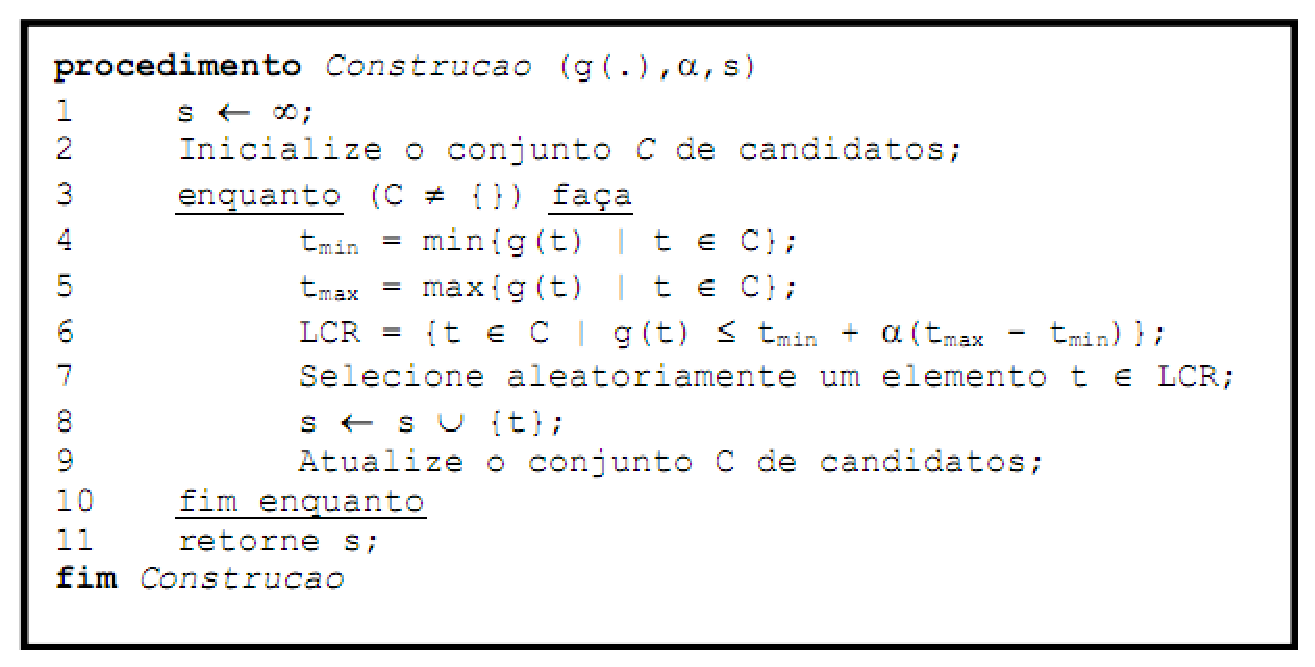
\includegraphics[scale=0.6]{graficos/grasp_construction_phase.eps}

%	\caption{pseudo-código da fase de construção da heurística GRASP}
%	\label{construction_phase}
%\end{figure}

\begin{figure}[H]
    \begin{center}
       \begin{tabular}{c} \hline
        \begin{lstlisting}[mathescape] 
		$\textit{procedimento}$ Construcao (g(.), $\alpha$, s)
		s $\leftarrow$ $\alpha$
		Inicialize o conjunto C de candidatos
		${\it enquanto}$ C $\neq$ { } ${\it faca}$
			$t_{min}$ = min{g(t) | $\in$ C}
			$t_{max}$ = max{g(t) | $\in$ C}
			LCR = {t $\in$ C | g(t) $\leq$ $t_{min}$ + $\alpha(t_{max} - t_{min}$)}
			Selecione aleatorimente um elemento t $\in$ LCR
			s $\leftarrow$ s $\cup$	{t}
			Atualize o conjunto C de candidatos
		${\it fim enquanto}$
		${\it retorne}$ s
		${\it fim}$ Construcao
	\end{lstlisting}\\
	\hline
 	\end{tabular}
     \end{center}
\caption{pseudo-código da fase de construção da heurística GRASP}
\label{construction_phase}
 \end{figure}


\section{Fase de Busca Local}
A fase de busca local está baseada na noção de vizinhança. A função N, a qual depende da estrutura do problema tratado, associa a cada solução viável s sua vizinhança N(s). Cada solução s' $\in$ N(s) é chamado de vizinho de s. É denominado movimento a modificação m que transforma uma solução s em outra s’, que esteja em sua vizinhança. Representa-se essa operação por s' $\leftarrow$ s $\in$ m. 
Em linhas gerais, a fase de busca local, começando de uma solução obtida pela fase de construção GRASP, navega pelo espaço de pesquisa passando de uma solução para outra, que seja sua vizinha, em busca de um ótimo local. 
A figura \ref{local_search_phase} descreve o pseudo-código de um algoritmo básico de busca local com respeito a uma certa vizinhança N(.) de s.

%\begin{figure}[H]
%	\centering
%	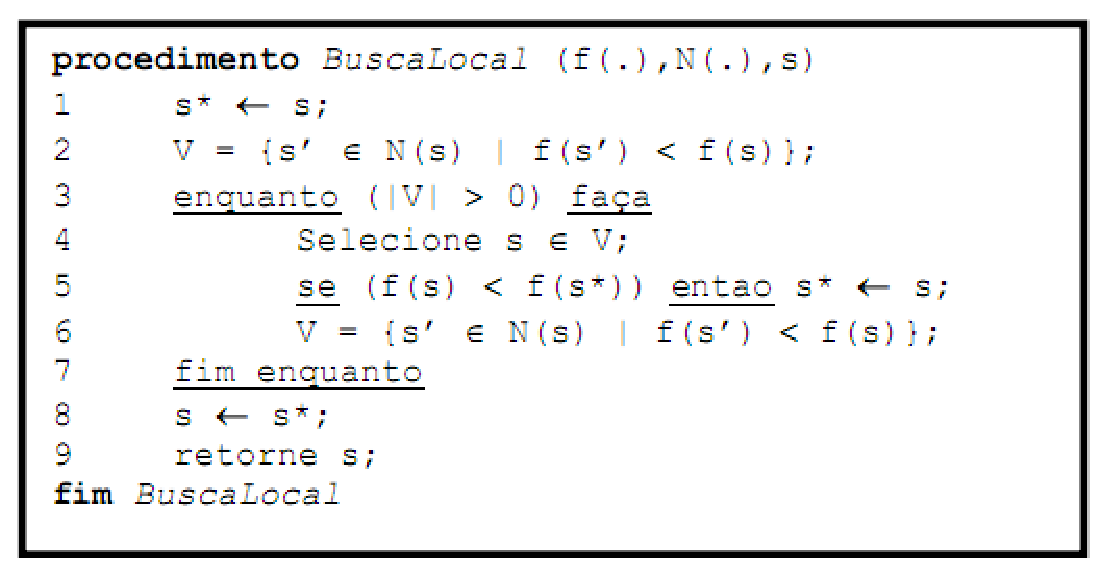
\includegraphics[scale=0.6]{graficos/grasp_local_search_phase.eps}
%	\caption{pseudo-código da fase de busca local da heurística GRASP}
%	\label{local_search_phase}
%\end{figure}

\begin{figure}[H]
    \begin{center}
       \begin{tabular}{c} \hline
        \begin{lstlisting}[mathescape] 
		$\textit{procedimento}$ BuscaLocal (f(.), N(.), s)
		$s^* \leftarrow$ s
		V = {s' $\in$ N(s) | f(s') < f(s)}
		${\it enquanto}$ (V > 0) ${\it faca}$
			selecione s $\in$ V
			${\it se}$ (f(s) < $f(s^*)$) ${\it entao}$
				$s^* \leftarrow$ s
			${\it fimse}$
			V = {s' $\in$ N(s) | f(s') < f(s)}
		${\it fim enquanto}$
		s $\leftarrow s^*$
		${\it retorne}$ s
		${\it fim}$ BuscaLocal
	\end{lstlisting}\\
	\hline
 	\end{tabular}
     \end{center}
\caption{pseudo-código da fase de busca local da heurística GRASP}
\label{local_search_phase}
 \end{figure}

